%--------------------------------------------------------------------------------------------------
\section{Geraden und Winkel}

\begin{center}
\begin{tikzpicture}[font=\small]
	\draw[mass] (1.3,0) arc[start angle=0, end angle=40, radius=1.3]; \node at (20:0.9) {$\alpha$};
	\draw[blue, very thick] (4.6,0) -- (0,0) -- (40:4.6);
	\fill (0,0) circle (2pt) node[above left] {$S$}; \fill (3.2,0) circle (2pt) node[below] {$A$}; \fill (40:3.2) circle (2pt) node[above left] {$B$};
	\node[align=center] (v) at (-2.2,-0.9) {vertex\\\color{black!60}Scheitel};
	\draw[-{Stealth}, thin] (v.east) -- (-0.15,-0.1);
	\node[align=center] (l) at (6.6,0.9) {arms (legs)\\\color{black!60}Schenkel};
	\draw[-{Stealth}, thin] (l.west) -- (4.3,0.1); \draw[-{Stealth}, thin] (l.west) -- ($(40:4.3)+(0.15,-0.1)$);
\end{tikzpicture}
\end{center}

\begin{lesen}
\lies{$g$}{the (straight) line $g$}{die Gerade $g$}
\lies{$\overline{AB}$}{the line segment $A$ $B$ \;/\; the distance from $A$ to $B$}{die Strecke $A$ $B$}
\lies{$g \parallel h$}{$g$ is parallel to $h$}{$g$ ist parallel zu $h$}
\lies{$g \perp h$}{$g$ is perpendicular to $h$ \;/\; $g$ is at right angles to $h$}{$g$ ist senkrecht zu $h$ \;/\; $g$ steht senkrecht auf $h$}
\lies{$\sphericalangle ASB$ \newline \footnotesize engl. $\angle ASB$}{angle $A$ $S$ $B$ (the vertex is named in the middle)}{Winkel $A$ $S$ $B$ (der Scheitel steht in der Mitte)}
\lies{$\alpha = 40\degree$}{alpha equals forty degrees: an acute angle}{Alpha gleich vierzig Grad: ein spitzer Winkel}
\lies{$\alpha + \beta = 90\degree$}{alpha and beta are complementary angles: they add up to ninety degrees}{Alpha und Beta sind Komplementwinkel: Sie ergänzen sich zu neunzig Grad}
\lies{$\alpha + \beta = 180\degree$}{alpha and beta are supplementary angles: they add up to one hundred and eighty degrees}{Alpha und Beta sind Supplementwinkel: Sie ergänzen sich zu hundertachtzig Grad}
\end{lesen}

\subsection*{Winkel an geschnittenen Parallelen}

\begin{center}
\begin{tikzpicture}[font=\small, scale=1.1]
	\coordinate (S1) at (0.6,2.2); \coordinate (S2) at (-0.67,0);
	\draw[red, thin] (S1) circle (0.42); \draw[red, thin] (S2) circle (0.42);
	\draw[blue, very thick] (-4,2.2) -- (4,2.2) node[right] {$g_1$};
	\draw[blue, very thick] (-4,0) -- (4,0) node[right] {$g_2$};
	\draw[blue, very thick] ($(S2)+(240:1.5)$) -- ($(S1)+(60:1.5)$) node[right] {$t$};
	\foreach \w/\n in {30/\alpha, 120/\beta, 210/\gamma, 300/\delta} {
		\node at ($(S1)+(\w:0.78)$) {$\n_1$}; \node at ($(S2)+(\w:0.78)$) {$\n_2$};}
	\node[align=left, anchor=west] at (5,1.1) {$g_1 \parallel g_2$\\ $t$: transversal\\\color{black!60}Transversale (schneidende Gerade)};
\end{tikzpicture}
\end{center}

\begin{lesen}
\lies{$\alpha_1$ und $\alpha_2$}{corresponding angles -- equal if the lines are parallel}{Stufenwinkel -- an Parallelen gleich groß}
\lies{$\gamma_1$ und $\alpha_2$}{alternate angles -- equal if the lines are parallel}{Wechselwinkel -- an Parallelen gleich groß}
\lies{$\delta_1$ und $\alpha_2$}{co-interior (allied) angles -- they add up to $180\degree$ if the lines are parallel}{entgegengesetzt liegende Winkel -- ergänzen sich an Parallelen zu $180\degree$}
\lies{$\alpha_1$ und $\gamma_1$}{vertically opposite angles -- always equal}{Scheitelwinkel -- immer gleich groß}
\lies{$\alpha_1$ und $\beta_1$}{adjacent angles on a straight line -- they add up to $180\degree$}{Nebenwinkel -- ergänzen sich zu $180\degree$}
\end{lesen}

\subsection*{Beispiele}

\begin{lesen}
\lies{$\alpha_1 = 65\degree$ \newline $\beta_1 = 180\degree - 65\degree = 115\degree$}{Alpha one is sixty-five degrees. Beta one is its adjacent angle on the straight line, so beta one is one hundred and fifteen degrees.}{Alpha eins beträgt fünfundsechzig Grad. Beta eins ist der Nebenwinkel, also hundertfünfzehn Grad.}
\lies{$\gamma_1 = \alpha_1 = 65\degree$}{Gamma one and alpha one are vertically opposite angles, so they are equal.}{Gamma eins und Alpha eins sind Scheitelwinkel, also gleich groß.}
\lies{$\alpha_2 = \alpha_1 = 65\degree$}{Alpha two and alpha one are corresponding angles on parallel lines, so they are equal.}{Alpha zwei und Alpha eins sind Stufenwinkel an Parallelen, also gleich groß.}
\lies{$\alpha = 90\degree$}{The lines $g$ and $h$ intersect at right angles.}{Die Geraden $g$ und $h$ schneiden einander rechtwinklig.}
\end{lesen}

%--------------------------------------------------------------------------------------------------
\section{Dreiecke, Vierecke und Vielecke}

\begin{center}
\begin{tikzpicture}[font=\small, scale=1.1]
	\draw[mass] (0.7,0) arc[start angle=0, end angle=59.04, radius=0.7]; \node at (28:0.45) {$\alpha$};
	\draw[mass] ($(5,0)+(136.85:0.7)$) arc[start angle=136.85, end angle=180, radius=0.7]; \node at ($(5,0)+(160:1.0)$) {$\beta$};
	\draw[mass] ($(1.8,3)+(239.04:0.6)$) arc[start angle=239.04, end angle=316.85, radius=0.6]; \node at ($(1.8,3)+(280:0.9)$) {$\gamma$};
	\draw[mass] (5.9,0) arc[start angle=0, end angle=136.85, radius=0.9]; \node at ($(5,0)+(60:1.2)$) {$\delta$};
	\draw[black!60, thick, dashed] (1.8,3) -- node[right, pos=0.6] {$h_c$} (1.8,0);
	\draw[black!60, thick] (2.15,0) arc[start angle=0, end angle=90, radius=0.35]; \fill[black!60] (1.95,0.15) circle (0.8pt);
	\draw[blue, very thick] (0,0) -- node[below] {$c$} (5,0) -- node[above right] {$a$} (1.8,3) -- node[above left] {$b$} cycle;
	\draw[blue, thick, dashed] (5,0) -- (6.6,0);
	\node[below left] at (0,0) {$A$}; \node[below] at (5,0) {$B$}; \node[above] at (1.8,3) {$C$};
	\node[align=left, anchor=west] at (7.4,2.2) {$a,\ b,\ c$: sides -- \color{black!60}Seiten};
	\node[align=left, anchor=west] at (7.4,1.6) {$\alpha,\ \beta,\ \gamma$: interior angles -- \color{black!60}Innenwinkel};
	\node[align=left, anchor=west] at (7.4,1.0) {$\delta$: exterior angle -- \color{black!60}Außenwinkel};
	\node[align=left, anchor=west] at (7.4,0.4) {$h_c$: height (altitude) -- \color{black!60}Höhe};
\end{tikzpicture}
\end{center}

\begin{lesen}
\lies{$\triangle ABC$}{triangle $A$ $B$ $C$}{Dreieck $A$ $B$ $C$}
\lies{$\alpha + \beta + \gamma = 180\degree$}{the interior angles of a triangle add up to one hundred and eighty degrees}{die Innenwinkel eines Dreiecks ergeben zusammen hundertachtzig Grad}
\lies{$\delta = \alpha + \gamma$}{an exterior angle equals the sum of the two opposite interior angles}{ein Außenwinkel ist so groß wie die beiden nicht anliegenden Innenwinkel zusammen}
\lies{$A = \dfrac{1}{2} \cdot c \cdot h_c$}{the area equals half the base times the height}{der Flächeninhalt ist gleich ein Halb mal Grundseite mal Höhe}
\lies{$a^2 + b^2 = c^2$}{$a$ squared plus $b$ squared equals $c$ squared -- Pythagoras' theorem: in a right-angled triangle the square on the hypotenuse equals the sum of the squares on the other two sides}{$a$ Quadrat plus $b$ Quadrat gleich $c$ Quadrat -- Satz des Pythagoras: Im rechtwinkligen Dreieck ist das Hypotenusenquadrat so groß wie die beiden Kathetenquadrate zusammen}
\lies{$\triangle ABC \cong \triangle DEF$}{triangle $A$ $B$ $C$ is congruent to triangle $D$ $E$ $F$}{Dreieck $A$ $B$ $C$ ist kongruent zu Dreieck $D$ $E$ $F$}
\lies{$\triangle ABC \sim \triangle PQR$}{triangle $A$ $B$ $C$ is similar to triangle $P$ $Q$ $R$}{Dreieck $A$ $B$ $C$ ist ähnlich zu Dreieck $P$ $Q$ $R$}
\end{lesen}

\subsection*{Besondere Dreiecke}

\begin{lesen}
\lies{\skGleichschenklig}{an isosceles triangle: two equal sides (the legs), the third side is the base; the two base angles are equal}{ein gleichschenkliges Dreieck: zwei gleich lange Seiten (Schenkel), die dritte Seite ist die Basis; die Basiswinkel sind gleich groß}
\lies{\skRechtwinklig}{a right-angled triangle (AE: right triangle): the two legs enclose the right angle, the hypotenuse lies opposite it}{ein rechtwinkliges Dreieck: Die Katheten schließen den rechten Winkel ein, die Hypotenuse liegt ihm gegenüber}
\end{lesen}

\begin{center}
\begin{tikzpicture}[font=\small, scale=1.0]
	\coordinate (A) at (0,0); \coordinate (B) at (3.6,0); \coordinate (C) at (1.8,3.118); \coordinate (M) at (1.8,1.039);
	\draw[red, thick] (M) circle (1.039); \draw[red, thick] (M) circle (2.078);
	\foreach \p/\q in {A/{2.7,1.559}, B/{0.9,1.559}, C/{1.8,0}} {\draw[black!60, dash dot] ($(\p)!-0.25!(\q)$) -- ($(\p)!1.45!(\q)$);}
	\draw[blue, very thick] (A) -- (B) -- (C) -- cycle; \fill (M) circle (2pt) node[right=2pt] {$M$};
	\node[align=left, anchor=west] at (5.2,3.1) {an equilateral triangle with its three axes of symmetry\\\color{black!60}ein gleichseitiges Dreieck mit seinen drei Symmetrieachsen};
	\node[align=left, anchor=west] at (5.2,1.9) {\textcolor{red}{incircle} and \textcolor{red}{circumcircle} --
		\color{black!60}Inkreis und Umkreis};
	\node[align=left, anchor=west, text width=10cm] at (5.2,0.2) {$M$ is the point of intersection of the altitudes, the perpendicular bisectors, the medians and the angle bisectors.\\\color{black!60}$M$ ist der Schnittpunkt der Höhen, der Mittelsenkrechten, der Seitenhalbierenden und der Winkelhalbierenden.};
\end{tikzpicture}
\end{center}

\subsection*{Vierecke und regelmäßige Vielecke}

\begin{lesen}
\lies{\skTrapez}{a trapezium (AE: trapezoid): a quadrilateral with one pair of parallel sides}{ein Trapez: ein Viereck mit einem Paar paralleler Seiten}
\lies{\skParallelogramm}{a parallelogram: a quadrilateral whose opposite sides are parallel}{ein Parallelogramm: ein Viereck, dessen gegenüberliegende Seiten parallel sind}
\lies{\skRaute}{a rhombus: a parallelogram with four equal sides}{eine Raute (ein Rhombus): ein Parallelogramm mit vier gleich langen Seiten}
\lies{\skRechteck}{a rectangle: a quadrilateral with four right angles}{ein Rechteck: ein Viereck mit vier rechten Winkeln}
\lies{\skQuadrat}{a square: a rectangle with four equal sides}{ein Quadrat: ein Rechteck mit vier gleich langen Seiten}
\lies{\skNeck{5} \skNeck{6} \skNeck{8}}{regular polygons: a pentagon, a hexagon and an octagon (all sides and all angles are equal)}{regelmäßige Vielecke: ein Fünfeck, ein Sechseck und ein Achteck (alle Seiten und alle Winkel sind gleich groß)}
\end{lesen}

\subsection*{Beispiele}

\begin{lesen}
\lies{$a = 3\,\mathrm{cm},\ b = 4\,\mathrm{cm}$ \newline $c = \sqrt{3^2 + 4^2}\,\mathrm{cm} = 5\,\mathrm{cm}$}{In a right-angled triangle the legs are three and four centimetres long. The hypotenuse is the square root of three squared plus four squared, that is five centimetres.}{In einem rechtwinkligen Dreieck sind die Katheten drei und vier Zentimeter lang. Die Hypotenuse ist die Wurzel aus drei Quadrat plus vier Quadrat, also fünf Zentimeter.}
\lies{$A = \frac12 \cdot 8\,\mathrm{cm} \cdot 5\,\mathrm{cm} = 20\,\mathrm{cm}^2$}{The area of the triangle is half of eight centimetres times five centimetres, which is twenty square centimetres.}{Der Flächeninhalt des Dreiecks ist ein Halb mal acht Zentimeter mal fünf Zentimeter, also zwanzig Quadratzentimeter.}
\lies{$u = 2 \cdot 6\,\mathrm{cm} + 2 \cdot 4\,\mathrm{cm} = 20\,\mathrm{cm}$}{The perimeter of a rectangle six centimetres long and four centimetres wide is twenty centimetres.}{Der Umfang eines Rechtecks mit sechs Zentimetern Länge und vier Zentimetern Breite beträgt zwanzig Zentimeter.}
\lies{$(6 - 2) \cdot 180\degree = 720\degree$}{The interior angles of a hexagon add up to seven hundred and twenty degrees.}{Die Innenwinkel eines Sechsecks ergeben zusammen siebenhundertzwanzig Grad.}
\end{lesen}

%--------------------------------------------------------------------------------------------------
\section{Der Kreis und seine Teile}

\begin{center}
\begin{tikzpicture}[font=\small, scale=1.2]
	\fill[gray!40] (120:2) arc[start angle=120, end angle=200, radius=2] -- cycle;
	\fill[blue!15] (0,0) -- (300:2) arc[start angle=300, end angle=345, radius=2] -- cycle;
	\draw[blue, very thick] (0,0) circle (2);
	\draw[blue, thick] (120:2) -- node[right, black, inner sep=2pt, pos=0.2] {$s$} (200:2);
	\draw[blue, thick] (300:2) -- (0,0) -- (345:2);
	\draw[black!70, thick] (90:2) -- node[left, pos=0.75] {$d$} (270:2);
	\draw[black!70, thick] (0,0) -- node[above] {$r$} (15:2);
	\draw[red, line width=2pt] (35:2) arc[start angle=35, end angle=75, radius=2]; \node[red] at (55:2.3) {$b$};
	\draw[red, thick] (-2.7,2) -- (2.7,2) node[right] {$t$};
	\fill[red] (0,2) circle (2pt) node[above] {$B$};
	\draw[red, thick] ($(215:2)!-0.5!(255:2)$) -- ($(215:2)!1.6!(255:2)$) node[right] {$g$};
	\fill (0,0) circle (2pt) node[left] {$M$};
	\node at (160:1.75) {$A_1$}; \node at (322:1.3) {$A_2$};
\end{tikzpicture}
\end{center}

\begin{lesen}
\lies{$M$}{the centre (AE: center)}{der Mittelpunkt}
\lies{$r$}{the radius \ipa{"reIdi@s} -- plural: radii \ipa{"reIdiaI}}{der Radius -- Plural: Radien}
\lies{$d = 2r$}{the diameter: the diameter is twice the radius}{der Durchmesser: Er ist doppelt so groß wie der Radius}
\lies{$s$}{a chord: a line segment joining two points on the circle}{eine Sehne: eine Strecke zwischen zwei Punkten des Kreises}
\lies{$g$}{a secant: a line cutting the circle in two points}{eine Sekante: eine Gerade, die den Kreis in zwei Punkten schneidet}
\lies{$t$, $B$}{a tangent: a line touching the circle at one point, the point of tangency (point of contact) $B$; the tangent is perpendicular to the radius at $B$}{eine Tangente: eine Gerade, die den Kreis in einem Punkt berührt, dem Berührungspunkt $B$; sie steht senkrecht auf dem Berührungsradius}
\lies{$b$}{an arc (of the circle)}{ein Kreisbogen}
\lies{$A_1$}{a segment: the region between a chord and an arc}{ein Kreisabschnitt (Kreissegment): die Fläche zwischen Sehne und Bogen}
\lies{$A_2$}{a sector: the region between two radii and an arc}{ein Kreisausschnitt (Kreissektor): die Fläche zwischen zwei Radien und einem Bogen}
\lies{$u = 2\pi r$}{the circumference equals two pi $r$}{der Umfang ist gleich zwei pi $r$}
\lies{$A = \pi r^2$}{the area equals pi $r$ squared}{der Flächeninhalt ist gleich pi $r$ Quadrat}
\end{lesen}

\subsection*{Beispiele}

\begin{lesen}
\lies{$r = 5\,\mathrm{cm}$ \newline $u = 2\pi \cdot 5\,\mathrm{cm} \approx 31{,}4\,\mathrm{cm}$}{The radius is five centimetres, so the circumference is two pi times five centimetres, which is approximately thirty-one point four centimetres.}{Der Radius beträgt fünf Zentimeter, also ist der Umfang zwei pi mal fünf Zentimeter, ungefähr einunddreißig Komma vier Zentimeter.}
\lies{$A = \pi \cdot (5\,\mathrm{cm})^2 \approx 78{,}5\,\mathrm{cm}^2$}{The area is pi times five centimetres squared, approximately seventy-eight point five square centimetres.}{Der Flächeninhalt ist pi mal fünf Zentimeter zum Quadrat, ungefähr achtundsiebzig Komma fünf Quadratzentimeter.}
\lies{$b = \dfrac{60\degree}{360\degree} \cdot 2\pi \cdot 5\,\mathrm{cm} \approx 5{,}24\,\mathrm{cm}$}{The arc belonging to an angle of sixty degrees is one sixth of the circumference, about five point two four centimetres.}{Der Bogen zu einem Winkel von sechzig Grad ist ein Sechstel des Umfangs, etwa fünf Komma zwei vier Zentimeter.}
\end{lesen}

%--------------------------------------------------------------------------------------------------
\section{Körper berechnen}

\begin{center}
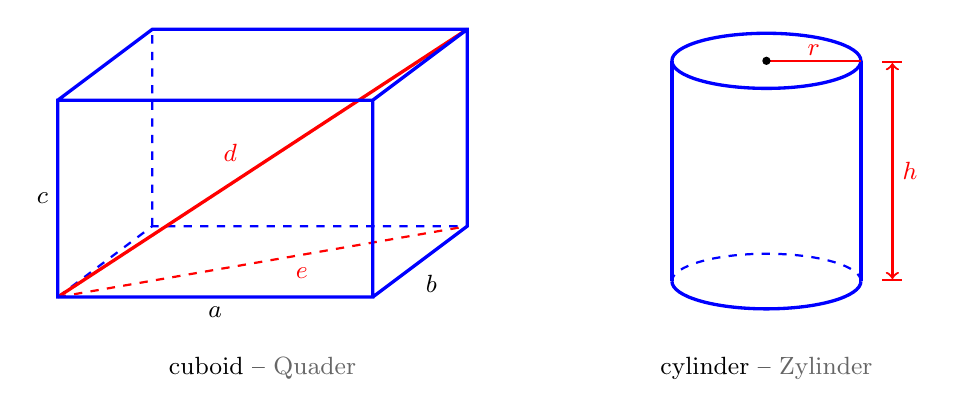
\begin{tikzpicture}[font=\small]
	\def\dx{1.2}\def\dy{0.9}
	\draw[blue, thick, dashed] (0,0) -- (\dx,\dy) -- (4+\dx,\dy) (\dx,\dy) -- (\dx,2.5+\dy);
	\draw[red, thick, dashed] (0,0) -- (4+\dx,\dy);
	\draw[red, very thick] (0,0) -- (4+\dx,2.5+\dy);
	\draw[blue, very thick] (0,0) rectangle (4,2.5) (4,0) -- (4+\dx,\dy) -- (4+\dx,2.5+\dy) -- (\dx,2.5+\dy) -- (0,2.5) (4,2.5) -- (4+\dx,2.5+\dy);
	\node[below] at (2,0) {$a$}; \node[below right] at (4.55,0.4) {$b$}; \node[left] at (0,1.25) {$c$};
	\node[red, above left] at (2.4,1.6) {$d$}; \node[red, below] at (3.1,0.5) {$e$};
	\node[align=center] at (2.6,-0.9) {cuboid -- \color{black!60}Quader};
	\begin{scope}[shift={(9,0.2)}]
		\draw[blue, thick, dashed] (1.2,0) arc[start angle=0, end angle=180, x radius=1.2, y radius=0.35];
		\draw[blue, very thick] (-1.2,0) arc[start angle=180, end angle=360, x radius=1.2, y radius=0.35];
		\draw[blue, very thick] (0,2.8) ellipse[x radius=1.2, y radius=0.35];
		\draw[blue, very thick] (-1.2,0) -- (-1.2,2.8) (1.2,0) -- (1.2,2.8);
		\draw[red, thick] (0,2.8) -- node[above, inner sep=1.5pt] {$r$} (1.2,2.8); \fill (0,2.8) circle (1.5pt);
		\draw[red, thick, |<->|] (1.6,0) -- node[right] {$h$} (1.6,2.8);
		\node[align=center] at (0,-1.1) {cylinder -- \color{black!60}Zylinder};
	\end{scope}
\end{tikzpicture}
\end{center}

\begin{lesen}
\lies{Quader}{A cuboid has eight vertices (corners), twelve edges and six faces.}{Ein Quader hat acht Ecken, zwölf Kanten und sechs Flächen.}
\lies{$e$, $d$}{$e$ is a face diagonal, $d$ is a space diagonal (body diagonal)}{$e$ ist eine Flächendiagonale, $d$ ist eine Raumdiagonale}
\lies{$V = a \cdot b \cdot c$}{the volume equals length times width times height}{das Volumen ist gleich Länge mal Breite mal Höhe}
\lies{$O = 2(ab + ac + bc)$}{the surface area equals two times the sum of $a$ $b$, $a$ $c$ and $b$ $c$}{der Oberflächeninhalt ist gleich zwei mal Klammer auf $a$ $b$ plus $a$ $c$ plus $b$ $c$ Klammer zu}
\lies{$V = a^3$}{the volume of a cube equals $a$ cubed}{das Volumen eines Würfels ist gleich $a$ hoch drei}
\lies{$V = \pi r^2 h$}{the volume of a cylinder equals pi $r$ squared $h$ (base area times height)}{das Volumen eines Zylinders ist gleich pi $r$ Quadrat $h$ (Grundfläche mal Höhe)}
\lies{$M = 2\pi r h$}{the curved surface area of a cylinder equals two pi $r$ $h$}{der Mantelflächeninhalt eines Zylinders ist gleich zwei pi $r$ $h$}
\lies{$V = \dfrac13 \cdot G \cdot h$}{the volume of a pyramid or a cone equals one third of the base area times the height}{das Volumen einer Pyramide oder eines Kegels ist gleich ein Drittel mal Grundfläche mal Höhe}
\lies{$V = \dfrac43 \pi r^3$}{the volume of a sphere equals four thirds pi $r$ cubed}{das Volumen einer Kugel ist gleich vier Drittel pi $r$ hoch drei}
\lies{$O = 4\pi r^2$}{the surface area of a sphere equals four pi $r$ squared}{der Oberflächeninhalt einer Kugel ist gleich vier pi $r$ Quadrat}
\end{lesen}

\subsection*{Besondere Körper}

\begin{lesen}
\lies{\skPyramidenstumpf \; \skKegelstumpf}{a frustum of a pyramid and a frustum of a cone (a truncated cone): the top has been cut off parallel to the base}{ein Pyramidenstumpf und ein Kegelstumpf: Die Spitze wurde parallel zur Grundfläche abgeschnitten}
\lies{\skTetraeder}{a tetrahedron: a regular polyhedron whose four faces are equilateral triangles}{ein (regelmäßiges) Tetraeder: ein Polyeder, dessen vier Flächen gleichseitige Dreiecke sind}
\lies{\skRotation}{a solid of revolution: it is generated by rotating a plane region about an axis -- here a semicircle generates a sphere}{ein Rotationskörper: Er entsteht, wenn eine ebene Fläche um eine Achse rotiert -- hier erzeugt ein Halbkreis eine Kugel}
\end{lesen}

\subsection*{Beispiele}

\begin{lesen}
\lies{$a = 4\,\mathrm{cm},\ b = 3\,\mathrm{cm},\ c = 2\,\mathrm{cm}$ \newline $V = 24\,\mathrm{cm}^3$}{The volume of the cuboid is four times three times two, that is twenty-four cubic centimetres.}{Das Volumen des Quaders ist vier mal drei mal zwei, also vierundzwanzig Kubikzentimeter.}
\lies{$O = 2 \cdot (12 + 8 + 6)\,\mathrm{cm}^2 = 52\,\mathrm{cm}^2$}{Its surface area is fifty-two square centimetres.}{Sein Oberflächeninhalt beträgt zweiundfünfzig Quadratzentimeter.}
\lies{$d = \sqrt{4^2 + 3^2 + 2^2}\,\mathrm{cm} = \sqrt{29}\,\mathrm{cm} \approx 5{,}39\,\mathrm{cm}$}{The space diagonal is the square root of twenty-nine, approximately five point three nine centimetres.}{Die Raumdiagonale ist die Wurzel aus neunundzwanzig, ungefähr fünf Komma drei neun Zentimeter.}
\lies{$r = 3\,\mathrm{cm},\ h = 10\,\mathrm{cm}$ \newline $V = \pi \cdot 9 \cdot 10\,\mathrm{cm}^3 \approx 282{,}7\,\mathrm{cm}^3$}{The volume of the cylinder is ninety pi, approximately two hundred and eighty-two point seven cubic centimetres.}{Das Volumen des Zylinders ist neunzig pi, ungefähr zweihundertzweiundachtzig Komma sieben Kubikzentimeter.}
\lies{$r = 3\,\mathrm{cm}$ \newline $V = \frac43 \pi \cdot 27\,\mathrm{cm}^3 \approx 113{,}1\,\mathrm{cm}^3$}{The volume of the sphere is thirty-six pi, approximately one hundred and thirteen point one cubic centimetres.}{Das Volumen der Kugel ist sechsunddreißig pi, ungefähr hundertdreizehn Komma eins Kubikzentimeter.}
\end{lesen}

%--------------------------------------------------------------------------------------------------
\section{Trigonometrie im Dreieck}

\begin{center}
\begin{tikzpicture}[font=\small, scale=1.1]
	\draw[mass] (1.3,0) arc[start angle=0, end angle=30.96, radius=1.3]; \node at (14:0.95) {$\alpha$};
	\draw[black!60, thick] (5,0.45) arc[start angle=90, end angle=180, radius=0.45]; \fill[black!60] (4.82,0.18) circle (1pt);
	\draw[mass] ($(5,3)+(210.96:0.8)$) arc[start angle=210.96, end angle=270, radius=0.8]; \node at ($(5,3)+(242:0.5)$) {$\beta$};
	\draw[blue, very thick] (0,0) -- (5,0) -- (5,3) -- cycle;
	\node[below left] at (0,0) {$A$}; \node[below right] at (5,0) {$C$}; \node[above right] at (5,3) {$B$};
	\node[align=center, above left] at (2.4,1.6) {$c$: hypotenuse\\\color{black!60}Hypotenuse};
	\node[align=left, right] at (5.15,1.5) {$a$: side opposite $\alpha$\\\color{black!60}Gegenkathete von $\alpha$};
	\node[align=center, below] at (2.5,-0.1) {$b$: side adjacent to $\alpha$\\\color{black!60}Ankathete von $\alpha$};
\end{tikzpicture}
\end{center}

\begin{lesen}
\lies{$\sin\alpha = \dfrac{a}{c}$}{sine alpha equals opposite over hypotenuse}{Sinus Alpha gleich Gegenkathete durch Hypotenuse}
\lies{$\cos\alpha = \dfrac{b}{c}$}{cosine alpha equals adjacent over hypotenuse}{Kosinus Alpha gleich Ankathete durch Hypotenuse}
\lies{$\tan\alpha = \dfrac{a}{b}$}{tan alpha equals opposite over adjacent}{Tangens Alpha gleich Gegenkathete durch Ankathete}
\lies{$\cot\alpha = \dfrac{b}{a}$}{cot alpha equals adjacent over opposite}{Kotangens Alpha gleich Ankathete durch Gegenkathete}
\lies{$\dfrac{a}{\sin\alpha} = \dfrac{b}{\sin\beta} = \dfrac{c}{\sin\gamma}$}{the sine rule (law of sines): $a$ over sine alpha equals $b$ over sine beta equals $c$ over sine gamma -- it holds in every triangle}{der Sinussatz: $a$ durch Sinus Alpha gleich $b$ durch Sinus Beta gleich $c$ durch Sinus Gamma -- er gilt in jedem Dreieck}
\lies{$c^2 = a^2 + b^2 - 2ab\cos\gamma$}{the cosine rule (law of cosines): $c$ squared equals $a$ squared plus $b$ squared minus two $a$ $b$ cosine gamma}{der Kosinussatz: $c$ Quadrat gleich $a$ Quadrat plus $b$ Quadrat minus zwei $a$ $b$ Kosinus Gamma}
\lies{$180\degree \mathrel{\widehat{=}} \pi$}{one hundred and eighty degrees corresponds to pi radians}{hundertachtzig Grad entsprechen pi im Bogenmaß}
\end{lesen}

\anmerkung{Englischsprachige Schülerinnen und Schüler merken sich die Definitionen mit dem Kunstwort
\textbf{SOH-CAH-TOA}: \textbf{S}ine = \textbf{O}pposite over \textbf{H}ypotenuse, \textbf{C}osine =
\textbf{A}djacent over \textbf{H}ypotenuse, \textbf{T}angent = \textbf{O}pposite over \textbf{A}djacent.
Die Tafelwerke mit Winkelfunktions- und Logarithmentafeln aus älteren Büchern ersetzt heute der
Taschenrechner (\textit{calculator}).}

\subsection*{Beispiele}

\begin{lesen}
\lies{$a = 3\,\mathrm{cm},\ c = 5\,\mathrm{cm}$ \newline $\sin\alpha = \frac35 = 0{,}6$ \newline $\alpha \approx 36{,}9\degree$}{Sine alpha equals three over five, which is nought point six. So alpha is the inverse sine of nought point six, approximately thirty-six point nine degrees.}{Sinus Alpha ist drei durch fünf, also null Komma sechs. Damit ist Alpha der Arkussinus von null Komma sechs, ungefähr sechsunddreißig Komma neun Grad.}
\lies{$\sin 30{,}2\degree \approx 0{,}5030$}{the sine of thirty point two degrees is approximately nought point five nought three nought}{der Sinus von dreißig Komma zwei Grad ist ungefähr null Komma fünf null drei null}
\lies{$h = 20\,\mathrm{m} \cdot \tan 35\degree \approx 14{,}0\,\mathrm{m}$}{From a point twenty metres away the top of a tree is seen at an angle of elevation of thirty-five degrees. The tree is about fourteen metres high.}{Aus zwanzig Metern Entfernung sieht man die Spitze eines Baumes unter einem Höhenwinkel von fünfunddreißig Grad. Der Baum ist etwa vierzehn Meter hoch.}
\lies{$a = 5,\ b = 7,\ \gamma = 60\degree$ \newline $c^2 = 25 + 49 - 70 \cdot \frac12 = 39$ \newline $c \approx 6{,}24$}{By the cosine rule, $c$ squared equals twenty-five plus forty-nine minus seventy times one half, which is thirty-nine. So $c$ is approximately six point two four.}{Nach dem Kosinussatz ist $c$ Quadrat gleich fünfundzwanzig plus neunundvierzig minus siebzig mal ein Halb, also neununddreißig. Damit ist $c$ ungefähr sechs Komma zwei vier.}
\lies{$a = 8,\ \alpha = 30\degree,\ \beta = 45\degree$ \newline $b = \dfrac{8 \cdot \sin 45\degree}{\sin 30\degree} \approx 11{,}31$}{By the sine rule, $b$ equals eight times sine forty-five degrees over sine thirty degrees, approximately eleven point three one.}{Nach dem Sinussatz ist $b$ gleich acht mal Sinus fünfundvierzig Grad durch Sinus dreißig Grad, ungefähr elf Komma drei eins.}
\end{lesen}

%--------------------------------------------------------------------------------------------------
\section{Koordinaten und Geraden}

\begin{center}
\begin{tikzpicture}[font=\small, scale=0.95]
	\draw[achse] (-0.7,0) -- (5.6,0) node[below left] {$x$}; \draw[achse] (0,-0.7) -- (0,4.2) node[below left] {$y$};
	\draw[mass] (1.2,0) arc[start angle=0, end angle=36.87, radius=1.2]; \node at (17:1.6) {$\varphi$};
	\draw[black!60, dashed] (4,0) node[below, black] {$x_P$} -- (4,3) -- (0,3) node[left, black] {$y_P$};
	\draw[red, very thick] (0,0) -- node[above left, inner sep=2pt] {$r$} (4,3);
	\fill (4,3) circle (2pt) node[above right] {$P$}; \node[below left] at (0,0) {$O$};
	\begin{scope}[shift={(9.6,0.3)}]
		\draw[achse] (-3.2,0) -- (6.2,0) node[below left] {$x$}; \draw[achse] (0,-0.9) -- (0,4.2) node[below left] {$y$};
		\draw[mass] (-1,0) arc[start angle=0, end angle=26.57, radius=1]; \node at ($(-2,0)+(12:1.4)$) {$\alpha$};
		\draw[blue, very thick] (-3,-0.5) -- (5.6,3.8) node[right] {$g$};
		\draw[black!60, thick] (2,2) -- node[below] {$\Delta x$} (4,2) -- node[right] {$\Delta y$} (4,3);
		\draw[red, thick, |<->|] (-0.3,0) -- node[left] {$n$} (-0.3,1);
		\fill[red] (0,1) circle (2pt);
	\end{scope}
\end{tikzpicture}
\end{center}

\begin{lesen}
\lies{$P(4 \mid 3)$ \newline \footnotesize engl. $P(4, 3)$}{the point $P$ four three: its $x$-coordinate (abscissa) is four, its $y$-coordinate (ordinate) is three}{der Punkt $P$ vier drei: Seine $x$-Koordinate (Abszisse) ist vier, seine $y$-Koordinate (Ordinate) ist drei}
\lies{$P(r;\,\varphi)$}{the polar coordinates of $P$: the distance $r$ from the origin (the pole) and the polar angle phi}{die Polarkoordinaten von $P$: der Abstand $r$ vom Ursprung (Pol) und der Polarwinkel Phi}
\lies{$x = r\cos\varphi,\ y = r\sin\varphi$}{$x$ equals $r$ cosine phi, $y$ equals $r$ sine phi}{$x$ gleich $r$ Kosinus Phi, $y$ gleich $r$ Sinus Phi}
\lies{$y = mx + n$}{the equation of a straight line in slope-intercept form: $y$ equals $m$ $x$ plus $n$}{die Normalform der Geradengleichung: $y$ gleich $m$ $x$ plus $n$}
\lies{$m = \dfrac{\Delta y}{\Delta x} = \tan\alpha$}{the gradient (slope) $m$ equals delta $y$ over delta $x$ (\glqq rise over run\grqq); it is the tangent of the angle of inclination alpha}{die Steigung $m$ ist gleich Delta $y$ durch Delta $x$; sie ist der Tangens des Steigungswinkels Alpha}
\lies{$n$}{the $y$-intercept: the line cuts the $y$-axis at the point $(0 \mid n)$}{der $y$-Achsenabschnitt: Die Gerade schneidet die $y$-Achse im Punkt $(0 \mid n)$}
\lies{$m_1 = m_2$}{parallel lines have the same gradient}{parallele Geraden haben die gleiche Steigung}
\lies{$m_1 \cdot m_2 = -1$}{two lines are perpendicular if the product of their gradients is minus one}{zwei Geraden sind zueinander senkrecht, wenn das Produkt ihrer Steigungen minus eins ist}
\end{lesen}

\subsection*{Beispiele}

\begin{lesen}
\lies{$A(1 \mid 2),\ B(3 \mid 6)$ \newline $m = \dfrac{6 - 2}{3 - 1} = 2$}{Find the equation of the line through $A$ and $B$. The gradient is six minus two over three minus one, which is two.}{Bestimme die Gleichung der Geraden durch $A$ und $B$. Die Steigung ist sechs minus zwei durch drei minus eins, also zwei.}
\lies{$2 = 2 \cdot 1 + n \ \Rightarrow\ n = 0$ \newline $y = 2x$}{Substitute the coordinates of $A$: $n$ equals zero. The equation of the line is $y$ equals two $x$.}{Setze die Koordinaten von $A$ ein: $n$ ist null. Die Geradengleichung lautet $y$ gleich zwei $x$.}
\lies{$\overline{AB} = \sqrt{2^2 + 4^2} = \sqrt{20} \approx 4{,}47$}{The distance between $A$ and $B$ is the square root of twenty, approximately four point four seven.}{Der Abstand von $A$ und $B$ ist die Wurzel aus zwanzig, ungefähr vier Komma vier sieben.}
\lies{$2x = -x + 6 \ \Rightarrow\ x = 2$ \newline $S(2 \mid 4)$}{The lines $y$ equals two $x$ and $y$ equals minus $x$ plus six intersect at the point $S$ two four.}{Die Geraden $y$ gleich zwei $x$ und $y$ gleich minus $x$ plus sechs schneiden einander im Punkt $S$ zwei vier.}
\end{lesen}

%--------------------------------------------------------------------------------------------------
\section{Kegelschnitte}

\begin{center}
\begin{tikzpicture}[font=\footnotesize, scale=0.95]
	\begin{scope}
		\draw[achse] (-1.7,0) -- (1.9,0) node[below] {$x$}; \draw[achse] (0,-1.7) -- (0,1.9) node[left] {$y$};
		\draw[blue, very thick] (0,0) circle (1.3);
		\draw[red, thick] (0,0) -- node[above left, inner sep=1pt] {$r$} (40:1.3); \fill (40:1.3) circle (1.5pt) node[above right] {$P$};
		\node[align=center] at (0,-2.3) {circle\\\color{black!60}Kreis};
	\end{scope}
	\begin{scope}[shift={(4.3,0)}]
		\draw[achse] (-2.1,0) -- (2.3,0) node[below] {$x$}; \draw[achse] (0,-1.7) -- (0,1.9) node[left] {$y$};
		\draw[blue, very thick] (0,0) ellipse[x radius=1.7, y radius=1.1];
		\coordinate (P) at ({1.7*cos(65)},{1.1*sin(65)});
		\draw[red, thick] (-1.296,0) -- (P) -- (1.296,0);
		\fill[red] (-1.296,0) circle (1.5pt) node[below] {$F_1$} (1.296,0) circle (1.5pt) node[below] {$F_2$};
		\fill (P) circle (1.5pt) node[above right] {$P$};
		\node[align=center] at (0,-2.3) {ellipse\\\color{black!60}Ellipse};
	\end{scope}
	\begin{scope}[shift={(8.9,0)}]
		\draw[achse] (-2.1,0) -- (2.3,0) node[below] {$x$}; \draw[achse] (0,-1.7) -- (0,1.9) node[left] {$y$};
		\draw[black!50, dashed] (-1.6,-1.6) -- (1.6,1.6) (-1.6,1.6) -- (1.6,-1.6);
		\draw[blue, very thick, domain=-1.5:1.5, samples=40, variable=\t] plot ({0.7*cosh(\t)}, {0.7*sinh(\t)});
		\draw[blue, very thick, domain=-1.5:1.5, samples=40, variable=\t] plot ({-0.7*cosh(\t)}, {0.7*sinh(\t)});
		\fill[red] (-0.99,0) circle (1.5pt) node[below left, inner sep=1pt] {$F_1$} (0.99,0) circle (1.5pt) node[below right, inner sep=1pt] {$F_2$};
		\node[align=center] at (0,-2.3) {hyperbola\\\color{black!60}Hyperbel};
	\end{scope}
	\begin{scope}[shift={(13.2,0)}]
		\draw[achse] (-1.2,0) -- (2.3,0) node[below] {$x$}; \draw[achse] (0,-1.7) -- (0,1.9) node[left] {$y$};
		\draw[blue, very thick, domain=-1.6:1.6, samples=40, variable=\t] plot ({\t*\t/1.6}, {\t});
		\draw[red, thick, dashed] (-0.4,-1.6) -- (-0.4,1.7) node[left] {$l$};
		\fill[red] (0.4,0) circle (1.5pt) node[below right, inner sep=1pt] {$F$};
		\node[align=center] at (0.5,-2.3) {parabola\\\color{black!60}Parabel};
	\end{scope}
\end{tikzpicture}
\end{center}

\begin{lesen}
\lies{$x^2 + y^2 = r^2$}{the equation of a circle with its centre at the origin and the radius $r$: $x$ squared plus $y$ squared equals $r$ squared}{die Gleichung eines Kreises um den Ursprung mit dem Radius $r$: $x$ Quadrat plus $y$ Quadrat gleich $r$ Quadrat}
\lies{$\dfrac{x^2}{a^2} + \dfrac{y^2}{b^2} = 1$}{the equation of an ellipse \ipa{I"lIps}: $x$ squared over $a$ squared plus $y$ squared over $b$ squared equals one; $a$ is the semi-major axis, $b$ the semi-minor axis}{die Gleichung einer Ellipse: $x$ Quadrat durch $a$ Quadrat plus $y$ Quadrat durch $b$ Quadrat gleich eins; $a$ ist die große, $b$ die kleine Halbachse}
\lies{$\overline{PF_1} + \overline{PF_2} = 2a$}{$F_1$ and $F_2$ are the foci \ipa{"f@UsaI} (singular: focus): for every point $P$ on the ellipse the sum of the distances from the foci is constant}{$F_1$ und $F_2$ sind die Brennpunkte: Für jeden Ellipsenpunkt $P$ ist die Summe der Abstände zu den Brennpunkten konstant}
\lies{$\dfrac{x^2}{a^2} - \dfrac{y^2}{b^2} = 1$}{the equation of a hyperbola \ipa{haI"p3:b@l@}: $x$ squared over $a$ squared minus $y$ squared over $b$ squared equals one; the dashed lines are its asymptotes}{die Gleichung einer Hyperbel: $x$ Quadrat durch $a$ Quadrat minus $y$ Quadrat durch $b$ Quadrat gleich eins; die gestrichelten Geraden sind ihre Asymptoten}
\lies{$y^2 = 2px$}{the equation of a parabola with its vertex at the origin: $y$ squared equals two $p$ $x$; $F$ is the focus, $l$ the directrix \ipa{d@"rektrIks}}{die Scheitelgleichung einer Parabel: $y$ Quadrat gleich zwei $p$ $x$; $F$ ist der Brennpunkt, $l$ die Leitlinie}
\lies{$\overline{PF} = \overline{Pl}$}{every point of the parabola is equidistant from the focus and the directrix}{jeder Parabelpunkt hat von Brennpunkt und Leitlinie den gleichen Abstand}
\end{lesen}

\anmerkung{Kreis, Ellipse, Parabel und Hyperbel heißen Kegelschnitte (\textit{conic sections}, kurz
\textit{conics}), weil sie entstehen, wenn eine Ebene einen Doppelkegel schneidet.}

\subsection*{Beispiele}

\begin{lesen}
\lies{$x^2 + y^2 = 25$ \newline $P(3 \mid 4)$: $9 + 16 = 25$ \checkmark}{The point $P$ three four lies on the circle, because three squared plus four squared equals twenty-five.}{Der Punkt $P$ drei vier liegt auf dem Kreis, denn drei Quadrat plus vier Quadrat ist fünfundzwanzig.}
\lies{$\dfrac{x^2}{25} + \dfrac{y^2}{9} = 1$ \newline $e = \sqrt{25 - 9} = 4$}{The semi-axes of the ellipse are five and three. The foci are at the points four nought and minus four nought.}{Die Halbachsen der Ellipse sind fünf und drei. Die Brennpunkte liegen bei $(4 \mid 0)$ und $(-4 \mid 0)$.}
\lies{$y^2 = 8x$ \newline $p = 4$}{The focus of the parabola is the point two nought; the directrix is the line $x$ equals minus two.}{Der Brennpunkt der Parabel ist $(2 \mid 0)$; die Leitlinie ist die Gerade $x$ gleich minus zwei.}
\end{lesen}

%--------------------------------------------------------------------------------------------------
\section{Folgen, Vektoren, Matrizen und Kombinatorik}

\subsection*{Folgen und Reihen}
\begin{lesen}
\lies{$a_n = a_1 + (n - 1) \cdot d$}{the $n$th term of an arithmetic sequence: $a$ sub $n$ equals $a$ one plus $n$ minus one, times $d$ ($d$ is the common difference)}{das $n$-te Glied einer arithmetischen Folge: $a$ $n$ gleich $a$ eins plus $n$ minus eins mal $d$}
\lies{$a_n = a_1 \cdot q^{\,n-1}$}{the $n$th term of a geometric sequence: $a$ sub $n$ equals $a$ one times $q$ to the power of $n$ minus one ($q$ is the common ratio)}{das $n$-te Glied einer geometrischen Folge: $a$ $n$ gleich $a$ eins mal $q$ hoch $n$ minus eins}
\lies{$\displaystyle\sum_{k=1}^{n} k = \frac{n(n + 1)}{2}$}{the sum from $k$ equals one to $n$ of $k$ equals $n$ times $n$ plus one, all over two}{die Summe über $k$ für $k$ von eins bis $n$ ist gleich $n$ mal $n$ plus eins, geteilt durch zwei}
\lies{$\displaystyle\sum_{k=0}^{\infty} q^k = \frac{1}{1 - q}$ \newline für $|q| < 1$}{the infinite geometric series converges if the absolute value of $q$ is less than one; otherwise it diverges}{die unendliche geometrische Reihe konvergiert, wenn der Betrag von $q$ kleiner als eins ist; sonst divergiert sie}
\end{lesen}

\subsection*{Vektoren und Matrizen}
\begin{lesen}
\lies{$\vec{a},\ |\vec{a}\,|$}{vector $a$; the magnitude (modulus) of vector $a$}{Vektor $a$; der Betrag von Vektor $a$}
\lies{$\vec{a} \cdot \vec{b}$}{$a$ dot $b$ -- the scalar product (dot product)}{$a$ mal $b$ -- das Skalarprodukt}
\lies{$\vec{a} \times \vec{b}$}{$a$ cross $b$ -- the vector product (cross product)}{$a$ kreuz $b$ -- das Vektorprodukt (Kreuzprodukt)}
\lies{$\vec{a} \perp \vec{b} \ \Leftrightarrow\ \vec{a} \cdot \vec{b} = 0$}{two vectors are perpendicular if and only if their scalar product is zero}{zwei Vektoren sind genau dann zueinander senkrecht, wenn ihr Skalarprodukt null ist}
\lies{$A = \begin{pmatrix} 1 & 2 & 3\\ 4 & 5 & 6 \end{pmatrix}$}{$A$ is a two by three matrix: it has two rows and three columns (plural of matrix: matrices \ipa{"meItrIsi:z})}{$A$ ist eine Zwei-Kreuz-Drei-Matrix: Sie hat zwei Zeilen und drei Spalten}
\lies{$a_{ij}$}{$a$ $i$ $j$: the element in row $i$ and column $j$}{$a$ $i$ $j$: das Element in Zeile $i$ und Spalte $j$}
\lies{$\det A$}{the determinant of $A$}{die Determinante von $A$}
\end{lesen}

\subsection*{Kombinatorik}
\begin{lesen}
\lies{$n!$}{$n$ factorial: the number of permutations of $n$ different elements}{$n$ Fakultät: die Anzahl der Permutationen von $n$ verschiedenen Elementen}
\lies{$\dbinom{n}{k}$}{$n$ choose $k$: the number of combinations of $k$ elements chosen from $n$ (without repetition)}{$n$ über $k$: die Anzahl der Kombinationen von $k$ aus $n$ Elementen (ohne Wiederholung)}
\lies{$\dfrac{n!}{(n - k)!}$}{the number of arrangements of $k$ elements taken from $n$, where the order matters}{die Anzahl der Variationen von $k$ aus $n$ Elementen (mit Beachtung der Reihenfolge)}
\end{lesen}

\subsection*{Beispiele}

\begin{lesen}
\lies{$3;\ 7;\ 11;\ 15;\ \ldots$ \newline $a_{10} = 3 + 9 \cdot 4 = 39$}{an arithmetic sequence with the first term three and the common difference four; the tenth term is thirty-nine}{eine arithmetische Folge mit dem Anfangsglied drei und der Differenz vier; das zehnte Glied ist neununddreißig}
\lies{$\vektor{1}{2}{3} \cdot \vektor{4}{-1}{2} = 4 - 2 + 6 = 8$}{the scalar product of the two vectors is eight}{das Skalarprodukt der beiden Vektoren ist acht}
\lies{$\begin{vmatrix} 1 & 2\\ 3 & 4 \end{vmatrix} = 1 \cdot 4 - 2 \cdot 3 = -2$}{the determinant equals one times four minus two times three, which is minus two}{die Determinante ist eins mal vier minus zwei mal drei, also minus zwei}
\lies{$4! = 4 \cdot 3 \cdot 2 \cdot 1 = 24$}{Four factorial is twenty-four: four books can be arranged on a shelf in twenty-four different ways.}{Vier Fakultät ist vierundzwanzig: Vier Bücher lassen sich auf vierundzwanzig Arten ins Regal stellen.}
\lies{$\dbinom{5}{2} = \dfrac{5 \cdot 4}{2} = 10$}{Five choose two is ten: there are ten ways of choosing two pupils from a group of five.}{Fünf über zwei ist zehn: Es gibt zehn Möglichkeiten, aus fünf Schülern zwei auszuwählen.}
\end{lesen}

%--------------------------------------------------------------------------------------------------
\section{Das griechische Alphabet}

Griechische Buchstaben werden im Englischen anders ausgesprochen als im Deutschen -- besonders
auffällig bei $\pi$, $\varphi$, $\chi$ und $\psi$.

\begin{center}
{\small\renewcommand{\arraystretch}{1.25}
\begin{tabular}{@{}c c l l @{\hspace{1.3cm}} c c l l@{}}
	\toprule
	\multicolumn{2}{@{}l}{\textbf{Zeichen}} & \textbf{Englisch} & \textbf{Deutsch} & \multicolumn{2}{l}{\textbf{Zeichen}} & \textbf{Englisch} & \textbf{Deutsch} \\ \midrule
	$\mathrm{A}$ & $\alpha$ & alpha \ipa{"\ae lf@} & Alpha & $\mathrm{N}$ & $\nu$ & nu \ipa{nju:} & Ny \\
	$\mathrm{B}$ & $\beta$ & beta \ipa{"bi:t@} & Beta & $\Xi$ & $\xi$ & xi \ipa{ksaI} & Xi \\
	$\Gamma$ & $\gamma$ & gamma \ipa{"g\ae m@} & Gamma & $\mathrm{O}$ & $o$ & omicron \ipa{@U"maIkr6n} & Omikron \\
	$\Delta$ & $\delta$ & delta \ipa{"delt@} & Delta & $\Pi$ & $\pi$ & pi \ipa{paI} & Pi \\
	$\mathrm{E}$ & $\varepsilon$ & epsilon \ipa{"epsIl6n} & Epsilon & $\mathrm{P}$ & $\varrho$ & rho \ipa{r@U} & Rho \\
	$\mathrm{Z}$ & $\zeta$ & zeta \ipa{"zi:t@} & Zeta & $\Sigma$ & $\sigma$ & sigma \ipa{"sIgm@} & Sigma \\
	$\mathrm{H}$ & $\eta$ & eta \ipa{"i:t@} & Eta & $\mathrm{T}$ & $\tau$ & tau \ipa{taU} & Tau \\
	$\Theta$ & $\vartheta$ & theta \ipa{"Ti:t@} & Theta & $\Upsilon$ & $\upsilon$ & upsilon \ipa{ju:p"saIl@n} & Ypsilon \\
	$\mathrm{I}$ & $\iota$ & iota \ipa{aI"@Ut@} & Jota & $\Phi$ & $\varphi$ & phi \ipa{faI} & Phi \\
	$\mathrm{K}$ & $\kappa$ & kappa \ipa{"k\ae p@} & Kappa & $\mathrm{X}$ & $\chi$ & chi \ipa{kaI} & Chi \\
	$\Lambda$ & $\lambda$ & lambda \ipa{"l\ae md@} & Lambda & $\Psi$ & $\psi$ & psi \ipa{psaI} & Psi \\
	$\mathrm{M}$ & $\mu$ & mu \ipa{mju:} & My & $\Omega$ & $\omega$ & omega \ipa{"@UmIg@} & Omega \\
	\bottomrule
\end{tabular}}
\end{center}

\subsection*{Beispiele}

\begin{lesen}
\lies{$\alpha,\ \beta,\ \gamma$}{alpha, beta and gamma are the interior angles of the triangle}{Alpha, Beta und Gamma sind die Innenwinkel des Dreiecks}
\lies{$\Delta x$}{delta $x$: the difference between two $x$-values}{Delta $x$: die Differenz zweier $x$-Werte}
\lies{$\varepsilon > 0$}{for every epsilon greater than zero}{für jedes Epsilon größer als null}
\lies{$\vec{x} = \vec{p} + \lambda \cdot \vec{u}$}{vector $x$ equals vector $p$ plus lambda times vector $u$}{Vektor $x$ gleich Vektor $p$ plus Lambda mal Vektor $u$}
\lies{$\mu = 3{,}5;\ \sigma \approx 1{,}71$}{the mean mu is three point five, the standard deviation sigma is approximately one point seven one}{der Erwartungswert My ist drei Komma fünf, die Standardabweichung Sigma ist ungefähr eins Komma sieben eins}
\lies{$\displaystyle\sum_{k=1}^{n} a_k$}{capital sigma: the sum of $a$ sub $k$ for $k$ from one to $n$}{groß Sigma: die Summe über $a$ $k$ für $k$ von eins bis $n$}
\lies{$\pi \approx 3{,}14$}{pi \ipa{paI} is approximately three point one four}{Pi ist ungefähr drei Komma eins vier}
\end{lesen}
